\begin{frame}{\textit{Socket Programming with TCP}}
  Modelagem
\end{frame}

\begin{frame}{Bases de dados}
  \begin{block}{INSS - Anuário Estatístico da Previdência Social}
    \begin{itemize}
      \item Dados Agregados
      \begin{itemize}
        \item Benefícios
        \item População 2013/2014/2015
      \end{itemize}
    \end{itemize}
  \end{block}
  \begin{figure}[h]
  	\begin{center}
      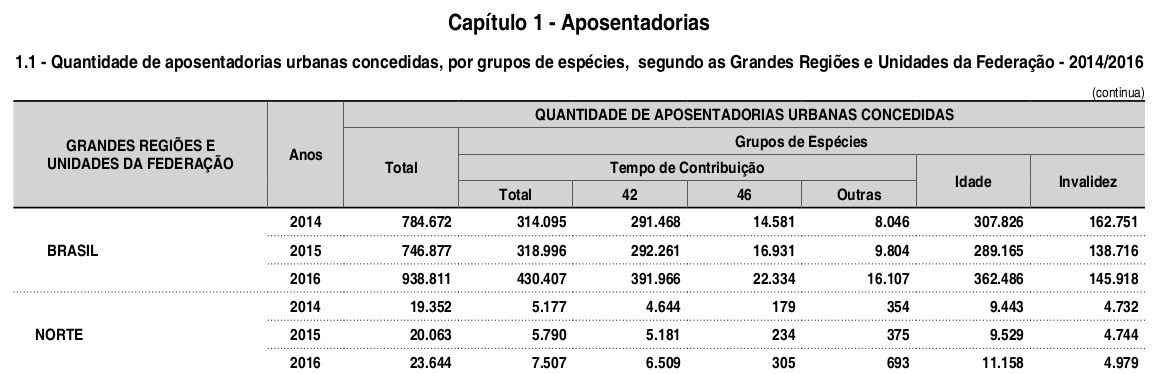
\includegraphics [scale=0.27]{./Figures/aeps01}
     % \caption {Estimativa de dispositivos conectados à Internet.}
  		%\label{fig:arq-imuno}
  	\end{center}
  \end{figure}
\end{frame}

\begin{frame}{Bases de dados}
  \begin{block}{Projeção da População Brasileira}
    \begin{itemize}
      \item Taxas anuais de crescimento da população até 2060
    \end{itemize}
  \end{block}
  \begin{figure}[h]
  	\begin{center}
      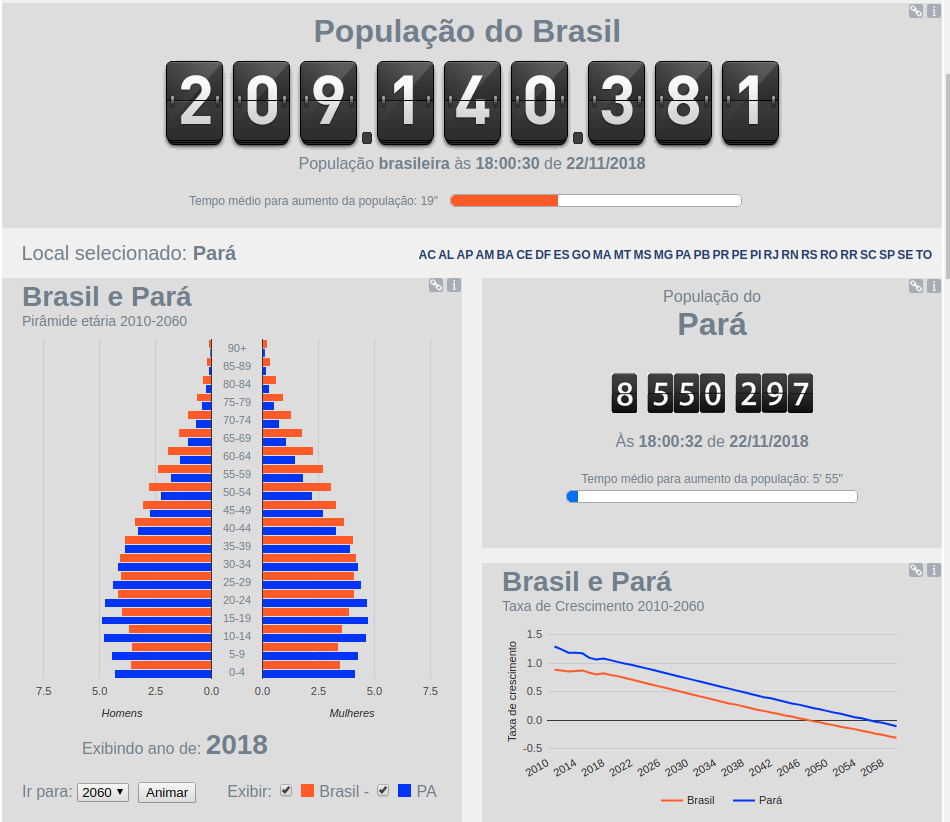
\includegraphics [scale=0.23]{./Figures/ibge-pop}
     % \caption {Estimativa de dispositivos conectados à Internet.}
  		%\label{fig:arq-imuno}
  	\end{center}
  \end{figure}
\end{frame}

\begin{frame}{Modelos de Projeção de Longo Prazo}
  \begin{block}{}
    \begin{itemize}
      \item Avaliação lida com eventos incertos e complexos sistemas
      interligados
      \item Modelo: representação simplificada da realidade, devendo
      considerar aspectos:
      \begin{itemize}
        \item demográficos
        \item financeiros
        \item institucionais
        \item jurídicos
      \end{itemize}
      \item Cálculo exige utilização de dados estatísticos confiáveis
    \end{itemize}
  \end{block}
\end{frame}

\begin{frame}{Variáveis em Modelos de Projeção}
\scriptsize
  \begin{block}{Variáveis Demográficas}
    \begin{itemize}
      \item Taxa de fecundidade
      \item Taxa de natalidade
      \item Expectativa de vida
      \item Taxa de migração
      \item Taxa de urbanização
    \end{itemize}
  \end{block}
  \pause
  \begin{block}{Variáveis Econômicas}
    \begin{itemize}
      \item Reajuste dos salários
      \item Inflação
      \item Taxas de juros
      \item Desemprego
      \item Produtividade
      \item Formalização
      \item Crescimento Econômico
    \end{itemize}
  \end{block}
\end{frame}

\begin{frame}{Variáveis em Modelos de Projeção}
  \begin{block}{Variáveis Previdenciárias}
    \begin{itemize}
      \item Alíquotas de contribuição
      \item Probabilidades de entrada no sistema
      \item Probabilidades de saída do sistema
      \item Reajuste dos benefícios
      \item Valores médios dos benefícios
    \end{itemize}
  \end{block}
\end{frame}

\begin{frame}{Modelos de Projeção}
  \begin{block}{1o Modelo Oficial do Governo Brasileiro}
    \begin{itemize}
      \item Criado no final da década de 90
      \item Permite projeção de receitas e despesas até a data de projeção da
      população (IBGE)
      \item Utilizado na elaboração de metas fiscais (LDO)
    \end{itemize}
  \end{block}

  \begin{block}{2o Modelo Oficial}
    \begin{itemize}
      \item Criado em 2016
      \item Visa melhor aderência a legislação vigente
      \item Modela de forma mais precisa os benefícios
      \item Mais complexo
    \end{itemize}
  \end{block}
\end{frame}

\begin{frame}{1o Modelo}
  \begin{block}{Considerações}
    \begin{itemize}
      \item Modelo determinístico
      \item  A LDO de 2017, não descreve quais benefícios são usados no modelo
      \item  A simplicidade do modelo o torna fácil de implementar, mas abstrair
      todos os benefícios em poucas equações afeta consideravelmente a
      precisão dos resultados
    \end{itemize}
  \end{block}
\end{frame}

\begin{frame}{1o Modelo - Estoque}
  \begin{block}{Estoque de Benefícios}
    \begin{itemize}
      \item Para cálculo das despesas, precisa-se calcular os \alert{benefícios
      ativos} no referido ano
      \item Calculado pelo método de fluxos, onde a concessão e cessação de
      benefícios são estimadas e utilizadas para definição do estoque
    \end{itemize}
  \end{block}
\end{frame}

\begin{frame}{1o Modelo - Estoque}
  \begin{block}{Fluxos de Concessão}
    \begin{center}
      $Fe(i,t,s,c,k) = P(i,t,s,c) \times Pe(i,t,s,c,k)$
    \end{center}
  \end{block}
  \begin{block}{Probabilidade de Entrada}
    \begin{center}
      $Pe(i,t,s,c,k) = \frac{concessoes(i,t,s,c,k)}{P(i,t,s,c)}$
    \end{center}
  \end{block}
  \begin{block}{Probabilidade de Sobrevivência}
    \begin{center}
      $Ps (i, t, s) = \frac{P(i+1, t+1, s)}{P(i,t,s)}$
    \end{center}
  \end{block}
\end{frame}

\begin{frame}{1o Modelo - Estoque}
  \begin{block}{Estoque de Benefício}
    \begin{center}
      $Eb(i, t, s, c, k) = Eb(i-1, t-1, s, c, k) \times Ps(i,s,c,k) \times
      Fe(i, t ,s, c, k)$
    \end{center}
  \end{block}
  \begin{block}{Estoque Total de Benefícios}
    \begin{center}
      $\sum_i \sum_s \sum_c \sum_k Eb(i,t,s,c,k)$
    \end{center}
  \end{block}
\end{frame}

\begin{frame}{1o Modelo - Despesa}
  \begin{block}{Despesa com Benefícios}
    Calculada a partir do estoque e do valor médio dos benefícios:
      \begin{center}
  \scriptsize
$Db(i,t,s,c,k) =$
$[Eb(i-1, t-1, s, c, k) \times Ps(i,s,c,k) \times Vmb(i,t,s,c,k)] + [Fe(i, t ,s, c, k) \times Vmbe(i,t,s,c,k)]$
      \end{center}
  \end{block}
  \scriptsize
    Onde:
    \begin{itemize}
      \item $Vmb$ é o valor médio atual do benefício (já concedido) pago
      \item $Vmbe$ é o valor médio do benefício (projetado) pago
    \end{itemize}
\end{frame}

\begin{frame}{1o Modelo - Receita}
  \begin{block}{Número de contribuintes}
  \scriptsize
      \begin{center}
      $\sum_i \sum_s \sum_c C(i,t,s,c) =$ \\
       $\sum_i \sum_s \sum_c P(i,t,s,c) \times Part(i,t,s,c) \times [1-Desemp(i,t,s,c)] \times d(i,t,s,c)$
      \end{center}
    %\end{itemize}
  \end{block}
  \scriptsize
    Onde:
    \begin{itemize}
      \item $C$ é o estoque de contibuintes
      \item $P$ é a população
      \item $Part$ é a taxa de participação na força de trabalho
      \item $Desemp$ é a taxa de desemprego
      \item $d$ é a densidade da contribuição (proporção de meses de contribuição do empregado no ano, onde $d=1$ significa 12 meses de contribuição
    \end{itemize}
\end{frame}

\begin{frame}{1o Modelo - Receita}
  \begin{block}{Valor da Receita $R$ no ano $t$}
  \scriptsize
      \begin{center}
    $R_t = \sum_i \sum_s \sum_c C(i,t,s,c) \times [al_{trab} \times \text{Min}(Teto, S_a(i,t,s,c)) + al_{emp} \times S_a(i,t,s,c)]$
      \end{center}
    %\end{itemize}
  \end{block}
  \scriptsize
    Onde:
    \begin{itemize}
      \item $al_{trab}$ é a alíquota de contribuição paga pelo trabalhador
      \item $al_{emp}$ é a alíquota de contribuição paga pelo empregador
      \item $Teto$ é o limite de contribuição (maior valor sobre o qual a alíquota pode incidir)
      \item $S_a$ é o saláro do empregado
    \end{itemize}
\end{frame}

%\begin{frame}
%  \begin{block}{}
%    \begin{itemize}
%      \item
%    \end{itemize}
%  \end{block}
%\end{frame}

%\begin{frame}
%  \begin{block}{}
%  \end{block}
%\end{frame}

%\begin{frame}
%  \begin{figure}[h]
%  	\begin{center}
%      \includegraphics [scale=0.3]{./Figures/Device-Estimates}
%     % \caption {Estimativa de dispositivos conectados à Internet.}
%  		%\label{fig:arq-imuno}
%  	\end{center}
%  \end{figure}
%\end{frame}

%\begin{frame}{Redes de Acesso}
%	\begin{figure}[!htb]
%		\centering
%		\subfloat[DSL]{
%			\includegraphics[height=3.5cm]{./Figures/DSLaccess}
%			\label{figdroopy}}
%		\quad %espaco separador
%		\subfloat[Cable]{
%			\includegraphics[height=3.5cm]{./Figures/CableAccess}
%			\label{figsnoop}}
%		%\caption{Subfiguras}
%		%\label{fig01}
%	\end{figure}
%\end{frame}

%\begin{frame}[fragile]
%\scriptsize
%\begin{verbatim}
%\end{verbatim}
%\end{frame}

%\begin{frame}{\textit{Socket Programming with TCP}}
%\scriptsize
%\lstinputlisting[language=Python, caption={TCP Server.}]{./code/upperServer/TCPserver.py}
%\end{frame}
